%%%%%%%%%%%%%%%%%%%%%%%%
%This tempelate is provided by Abdorrahman Mehri Ghahfarrokhi, petroleum university of technology, department of energy economics.
%email address: amehri.ghahfarrokhi@gmail.com
%%%%%%%%%%%%%%%%%%%%%%%%%

\RequirePackage[utf8]{inputenc}
\RequirePackage[T1]{fontenc}
\documentclass [xcolor=svgnames, t] {beamer} 
\usepackage[utf8]{inputenc}
\usepackage{booktabs, comment}
%\usepackage[slovak]{babel}
\usepackage[absolute, overlay]{textpos} 
\usepackage{pgfpages}
\usepackage[font=footnotesize]{caption}
\useoutertheme{infolines} 

\definecolor{red}{RGB}{250,0,75}
\setbeamercolor{title in head/foot}{bg=red, fg=white}
\setbeamercolor{author in head/foot}{bg=myuniversity}
\setbeamertemplate{page number in head/foot}{}
\usepackage{csquotes}


\usepackage{amsmath}
\usepackage[makeroom]{cancel}


\usepackage{textpos}

\usepackage{tikz}
\usepackage{algpseudocode}  % part of algorithmicx package
\usepackage{algorithm}

\usetheme{Madrid}
\definecolor{myuniversity}{RGB}{0, 85, 150}
\usecolortheme[named=myuniversity]{structure}
\usepackage{tikz}

\newtheorem{defn}{Definition}[section]
\newtheorem{thm}{Theorem}[section]
\newtheorem{claim}{Claim}[section]


\newtheorem{Shap}{Shapleyho hodnota}[section]
\newtheorem{Vektor}{\textbf{Vektorový prostor $\Gamma^n$}}[section]
\newtheorem{Trh}{Trh}[section]
\newtheorem{Obchod}{Obchod}[section]
\newtheorem{Volhra}{Volební hra}[section]

\newtheorem{Jednohlas}{\textbf{Shapleyho hodnota jednohlasných her}}[section]
\newtheorem{Jadro}{Jadro}[section]

\newtheorem{Lemke}{Lemke-Howson algorithm}[section]
\newtheorem{Nic}{}[section]
\def\QQ{\mathbb{Q}}
\def\RR{\mathbb{R}}
\def\ZZ{\mathbb{Z}}
\def\NN{\mathbb{N}}

\algnewcommand\algorithmicswitch{\textbf{switch}}
\algnewcommand\algorithmiccase{\textbf{case}}
\algnewcommand\algorithmicassert{\texttt{assert}}
\algnewcommand\Assert[1]{\State \algorithmicassert(#1)}%
% New "environments"
\algdef{SE}[SWITCH]{Switch}{EndSwitch}[1]{\algorithmicswitch\ #1\ \algorithmicdo}{\algorithmicend\ \algorithmicswitch}%
\algdef{SE}[CASE]{Case}{EndCase}[1]{\algorithmiccase\ #1}{\algorithmicend\ \algorithmiccase}%
\algtext*{EndSwitch}%
\algtext*{EndCase}%



\title[Optimisation algorithms powered by LLMs]{Optimisation algorithms powered by LLMs}
\institute[]{Pavol Jozef Šafárik University in Košice \\ Institute of Computer Science}
\titlegraphic{
\includegraphics[height=1.95cm]{picture/logopfupjsf.jpg}}
\author[Mgr. N. Micheľ]{
	\\ Mgr. Norbert Micheľ \\
    Supervisor:
    \\
    prof. RNDr. Gabriel Semanišin, PhD.
    }

\date{June 2026}

\addtobeamertemplate{navigation symbols}{}{%
    \usebeamerfont{footline}%
    \usebeamercolor[fg]{footline}%
    \hspace{1em}%
    \insertframenumber/\inserttotalframenumber
}

\begin{document}
\begin{frame}
\maketitle
\end{frame}

%%%%%%%%%%%%%%%%%%%%%%%%%%%%
%\logo{
\includegraphics[scale=0.14]{upjs-logo.png}}

%%%%%%%%%%%%%%%%%%%%%%%%%%

\begin{frame}
\frametitle{Contents}
\tableofcontents
\end{frame}


\section{Study and Teaching Activities}
\begin{frame}{Teaching Activities}
\begin{columns}[T]
    \begin{column}{0.62\textwidth} % Mierne zúžené, aby mal pravý stĺpec viac miesta
        \begin{itemize}
            \item \textbf{Course:} Programovací jazyk Python (Python programming language)
            \item \textbf{Objective:} Teaching students the fundamentals of Python programming
            \item \textbf{Responsibilities:}
            \begin{itemize}
                \item Lab assistance and student consulting
                \item Grading homework assignments and exams
            \end{itemize}
            \vfill
            \item \textbf{Status:}
            \begin{itemize}
                \item {\color{green!60!black}Finished} -- all students have successfully completed the course
            \end{itemize}
        \end{itemize}
    \end{column}

    \begin{column}{0.33\textwidth} % Rozšírené pre väčšie obrázky
        \centering
        \vspace{1em}
        
\includegraphics[width=0.7\textwidth]{figures/python.png} 
        
        \vfill % Týmto zatlačíme mačičku úplne na spodok slajdu
        
        \hfill % Posunie mačičku čo najviac doprava v rámci stĺpca
        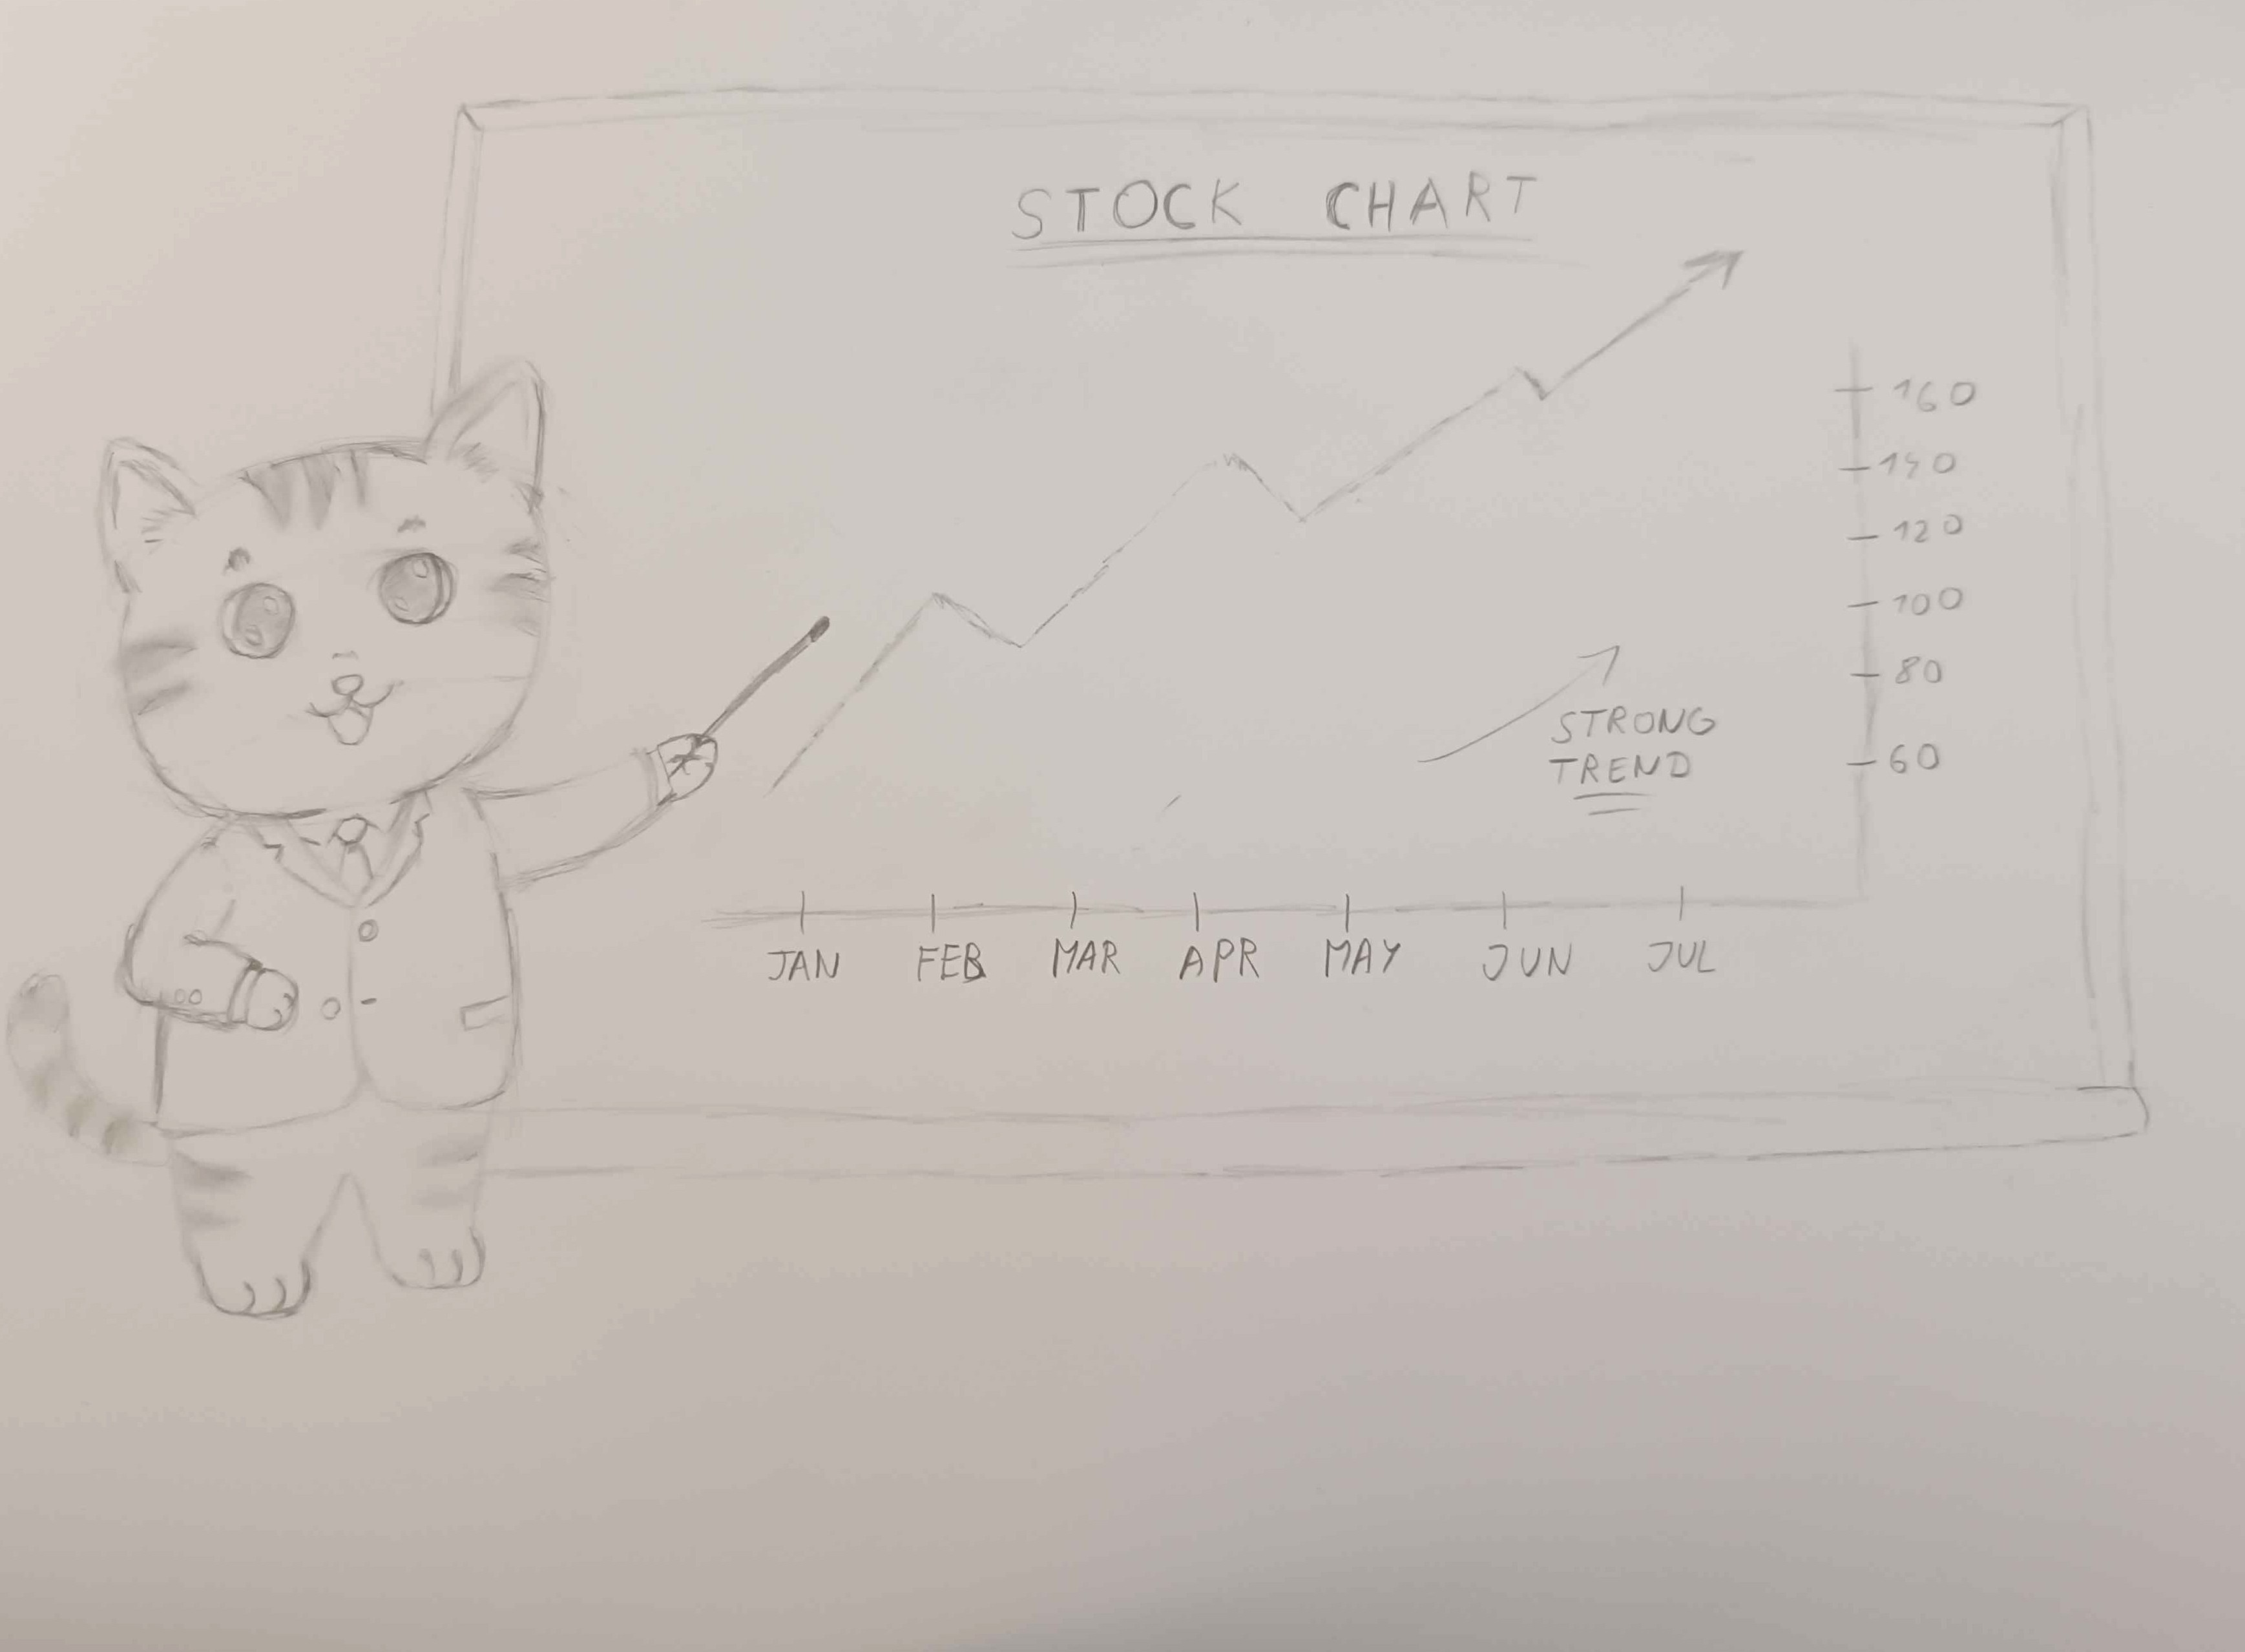
\includegraphics[width=1.1\textwidth]{figures/macicka.jpg} 
    \end{column}
\end{columns}
\end{frame}

\begin{frame}{Study Activities}
\begin{itemize}
    \item \textbf{Required Courses}
    \begin{itemize}
        \item English for PhD Students 1 -- {\color{green!60!black}passed}
        \item English for PhD Students 2 -- {\color{blue}in progress}
    \end{itemize}
    \item \textbf{Optional Courses}
    \begin{itemize}
        \item Methods of Machine Learning and Artificial Intelligence -- {\color{green!60!black}passed}
        \item Probabilistic and Approximation Algorithms and Heuristics -- {\color{blue}in progress}
        \item Theoretical Aspects of Neural Networks -- {\color{green!60!black}passed}
        \item Computational Complexity and Models -- {\color{green!60!black}passed}
    \end{itemize}
\end{itemize}

\vfill

\begin{center}
    \textbf{Plan:} Completion of all coursework requirements by the end of June.
\end{center}
\end{frame}

\section{Supervision and Consulting}
\begin{frame}{Supervision and Consulting}
\textbf{Topic:} Algorithms for Move Generation and Evaluation in Chess \\
\textbf{Role:} Consultant \hfill \textbf{Student:} Tomáš Oltman \\
\textbf{Thesis Defense Date:} 18.6.2026

\vfill % Pekne oddelí hlavičku od stĺpcov

\begin{columns}[T]
    \begin{column}{0.53\textwidth}
        \textbf{Key Implemented Algorithms:}
        \begin{itemize}
            \item \textbf{Quiescence Search} -- Prevents the horizon effect by extending the search for unstable positions.
            \item \textbf{Piece-Square Tables} -- Positional evaluation based on optimal square coordinates.
            \item \textbf{Zobrist Hashing} -- Enables fast transposition table lookups to eliminate redundant calculations.
        \end{itemize}
    \end{column}
    
    \begin{column}{0.45\textwidth} % Mierne rozšírené pre lepší komfort textu
        \begin{exampleblock}{Performance \& Rating}
            \begin{itemize}
                \item \textbf{Elo Rating:} $\approx \mathbf{1700}$
                \item \textbf{Human Equivalent:} Club player with \textbf{2 years} of active training.
                \item \textbf{Percentile:} Outperforms approximately \textbf{99\% of casual chess players}
            \end{itemize}
        \end{exampleblock}
    \end{column}
\end{columns}
\end{frame}



























\section{Conferences}


\begin{frame}{Spring School for PhD Students}

\begin{itemize}
    \item \textbf{Date:} May 25 – May 28, 2026
    \item \textbf{Location:} Stará Lesná, Slovakia (Congress Centre SAV Academia)
    \item \textbf{Event:} 12th annual university-wide conference for doctoral students
    \item \textbf{Activity:} Presentation of current scientific research results and multidisciplinary networking
\end{itemize}

\vfill

\begin{columns}[c]
    \begin{column}{0.7\textwidth}
        \centering
        % Oficiálne logo univerzity
        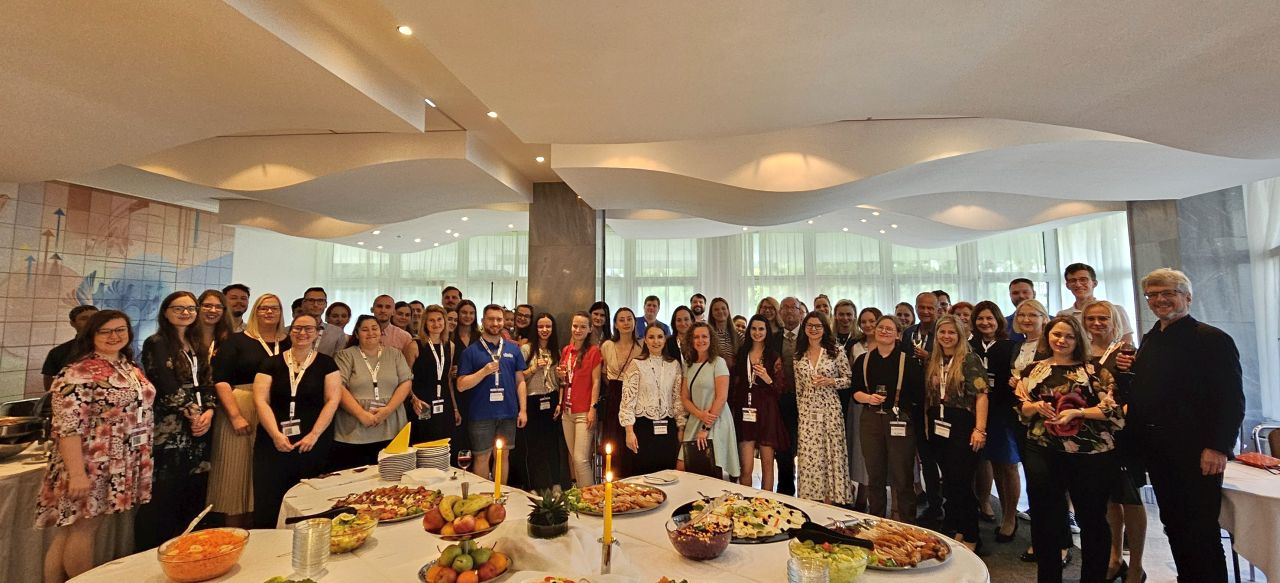
\includegraphics[width=0.9\textwidth]{figures/vsetcijar.jpg}
    \end{column}
    
    \begin{column}{0.3\textwidth}
        \centering
        % Fotka miesta konania (Vysoké Tatry / Stará Lesná)
        
\includegraphics[width=\textwidth]{figures/jarna_skola.jpg}
    \end{column}
\end{columns}
\end{frame}

\begin{frame}{Spring School for PhD Students -- Quiz Night}
\begin{itemize}
    \item \textbf{Format:} 70 questions covering various trivia topics
    \item \textbf{1st Place Score:} 60 / 70
    \item \textbf{Our Team Score:} 58 / 70
    \item \textbf{Final Ranking:} Secured \textbf{3rd place} overall
    \item \textbf{Key Highlight:} Defeated the professors' team (57 / 70)
\end{itemize}

\vfill

\begin{center}
    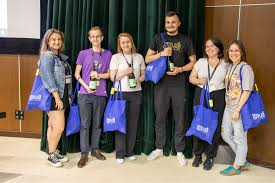
\includegraphics[width=0.45\textwidth]{figures/vysledky.jpg}
\end{center}
\end{frame}

\begin{frame}{Czech-Slovak Conference Graphs -- Academic Part}

\begin{itemize}
    \item \textbf{Date:} June 1 -- June 5, 2026
    \item \textbf{Location:} Zemplínska šírava, Slovakia
    \item \textbf{Focus:} Specialized conference focusing on graph theory and combinatorics.
    \item \textbf{Presentation:} Min cut-path problem
    \item \textbf{Post-Conference Follow-up:} 
    \begin{itemize}
        \item Received an email from one of the participants after the conference
        \item Shared a relevant research paper where a similar problem was solved
    \end{itemize}
\end{itemize}

\vfill
\hfill

\includegraphics[width=0.6\textwidth]{figures/csgt_logo.png}
\end{frame}


\begin{frame}{Czech-Slovak Conference Graphs -- Behind the Scenes}
\centering 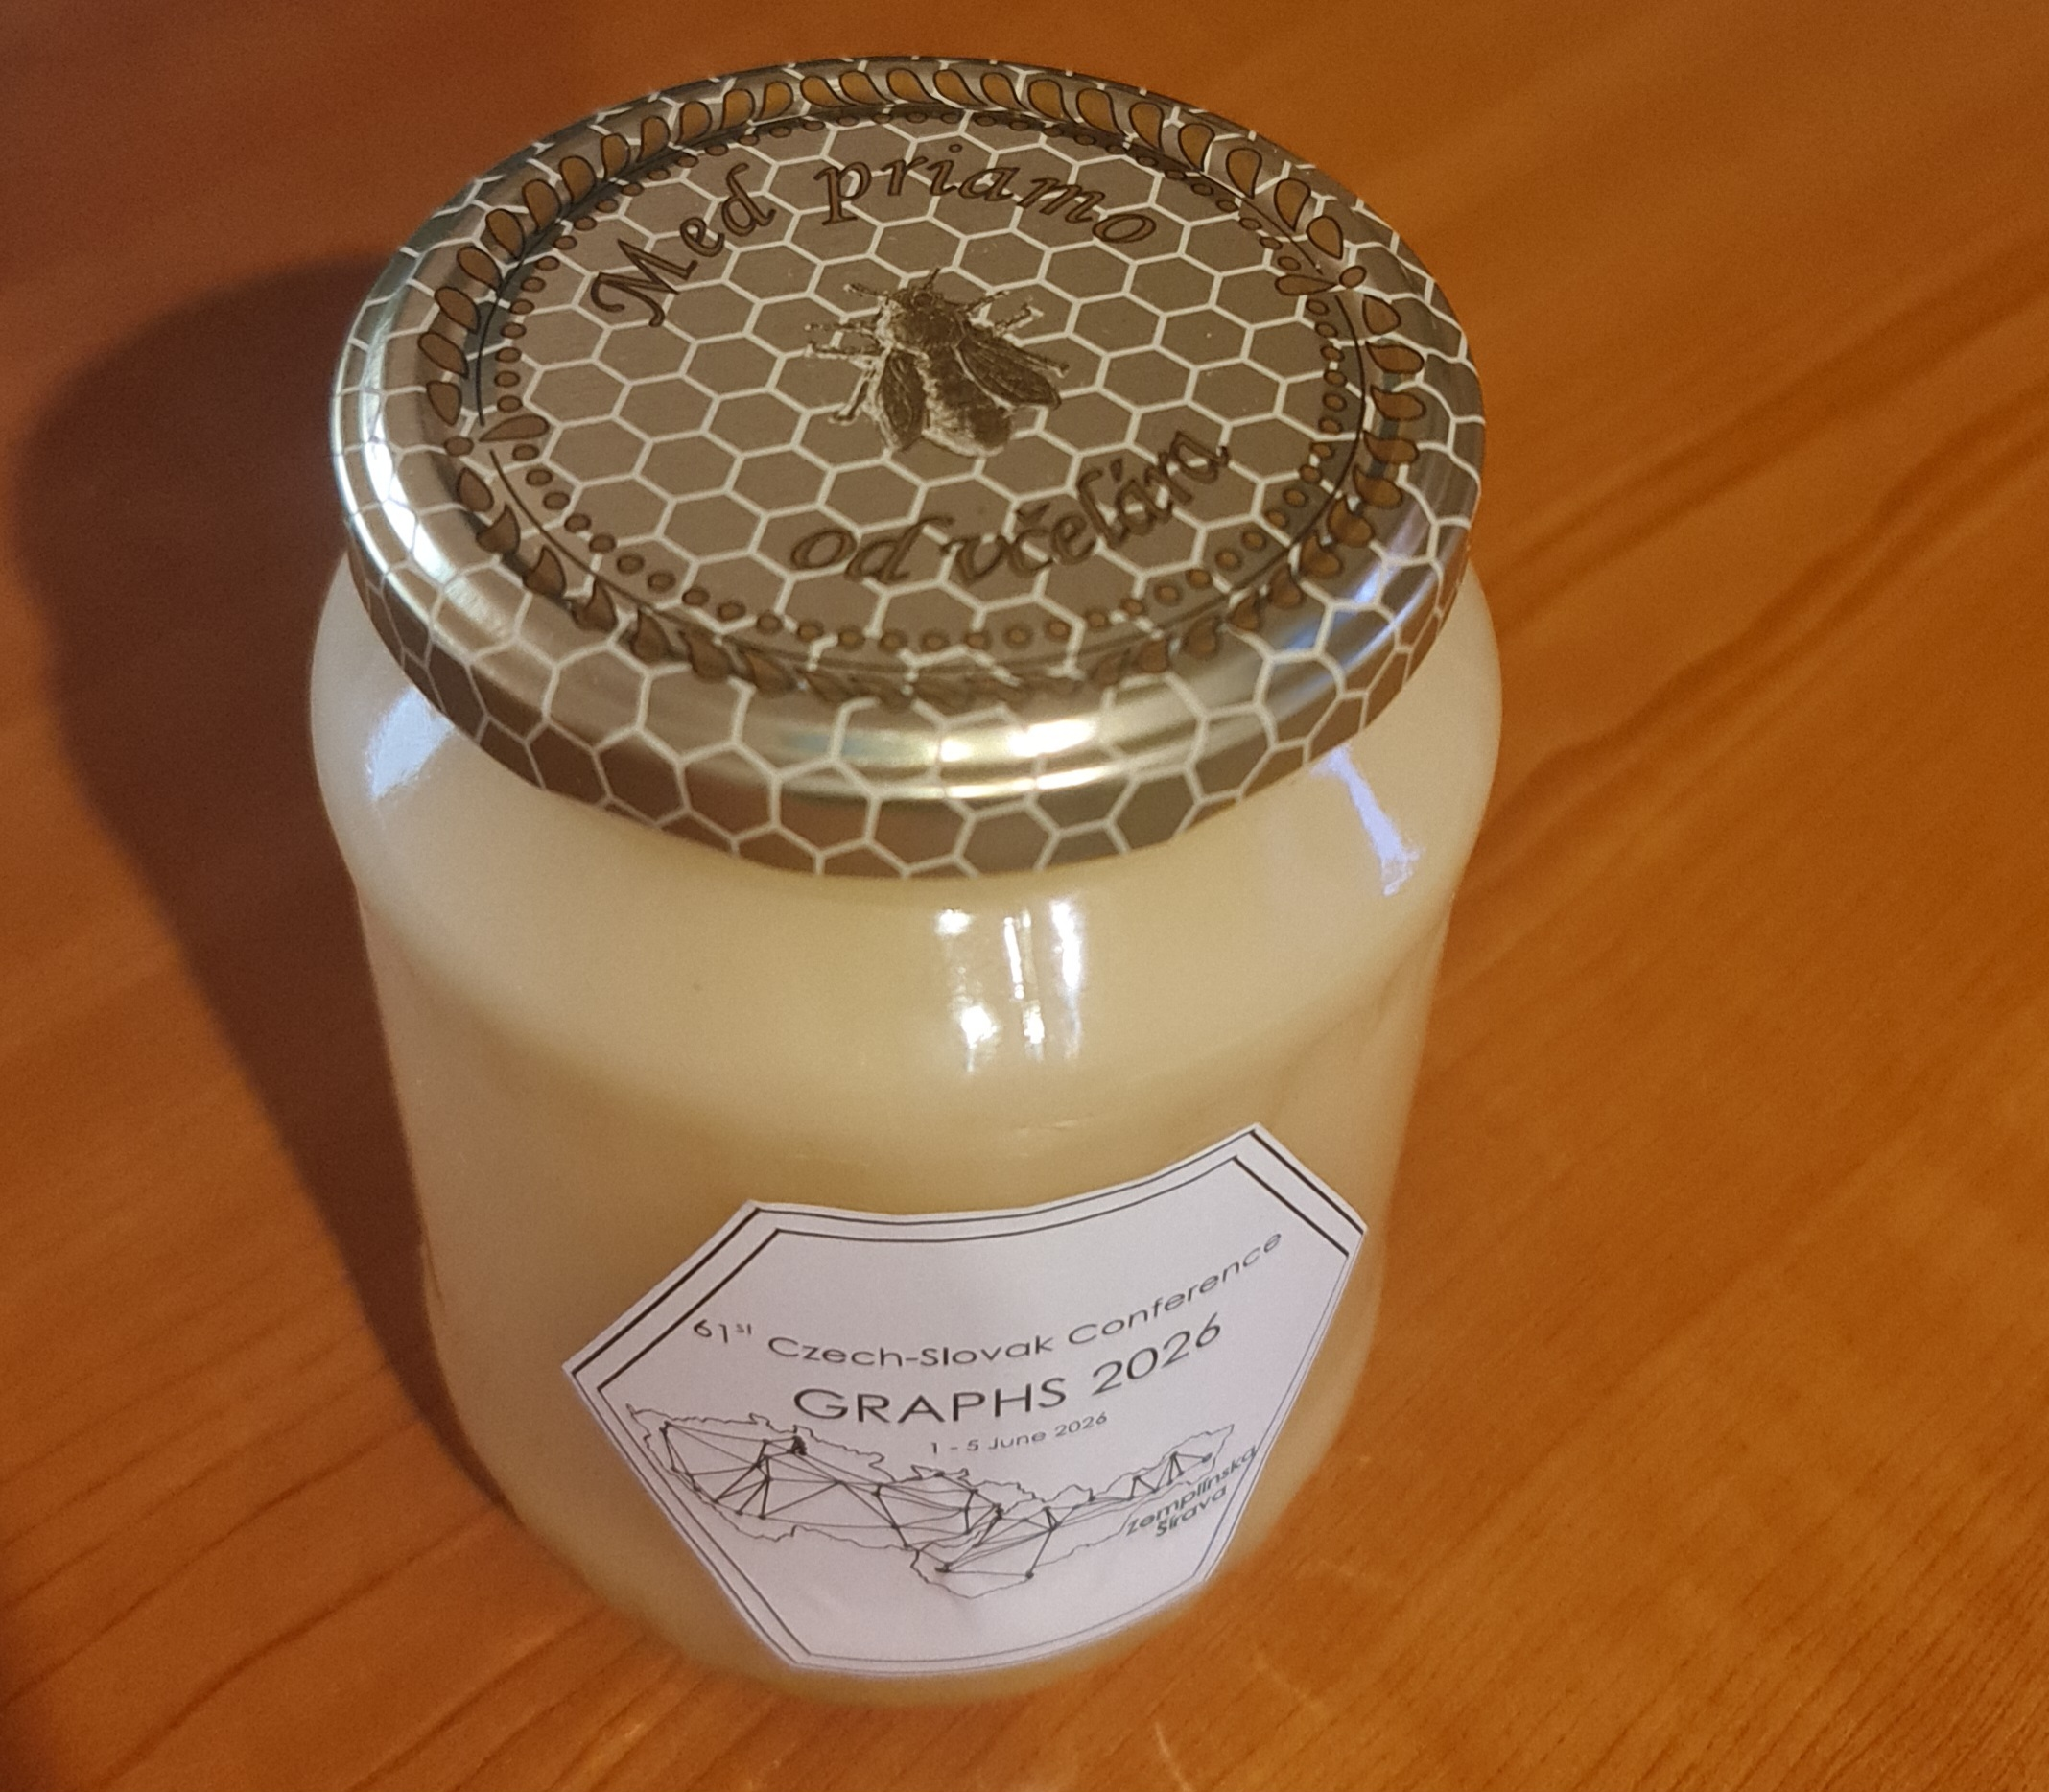
\includegraphics[width=0.75\textwidth]{figures/med.jpg} 
\end{frame}

\begin{frame}{Czech-Slovak Conference Graphs -- Trip}
\begin{center}
    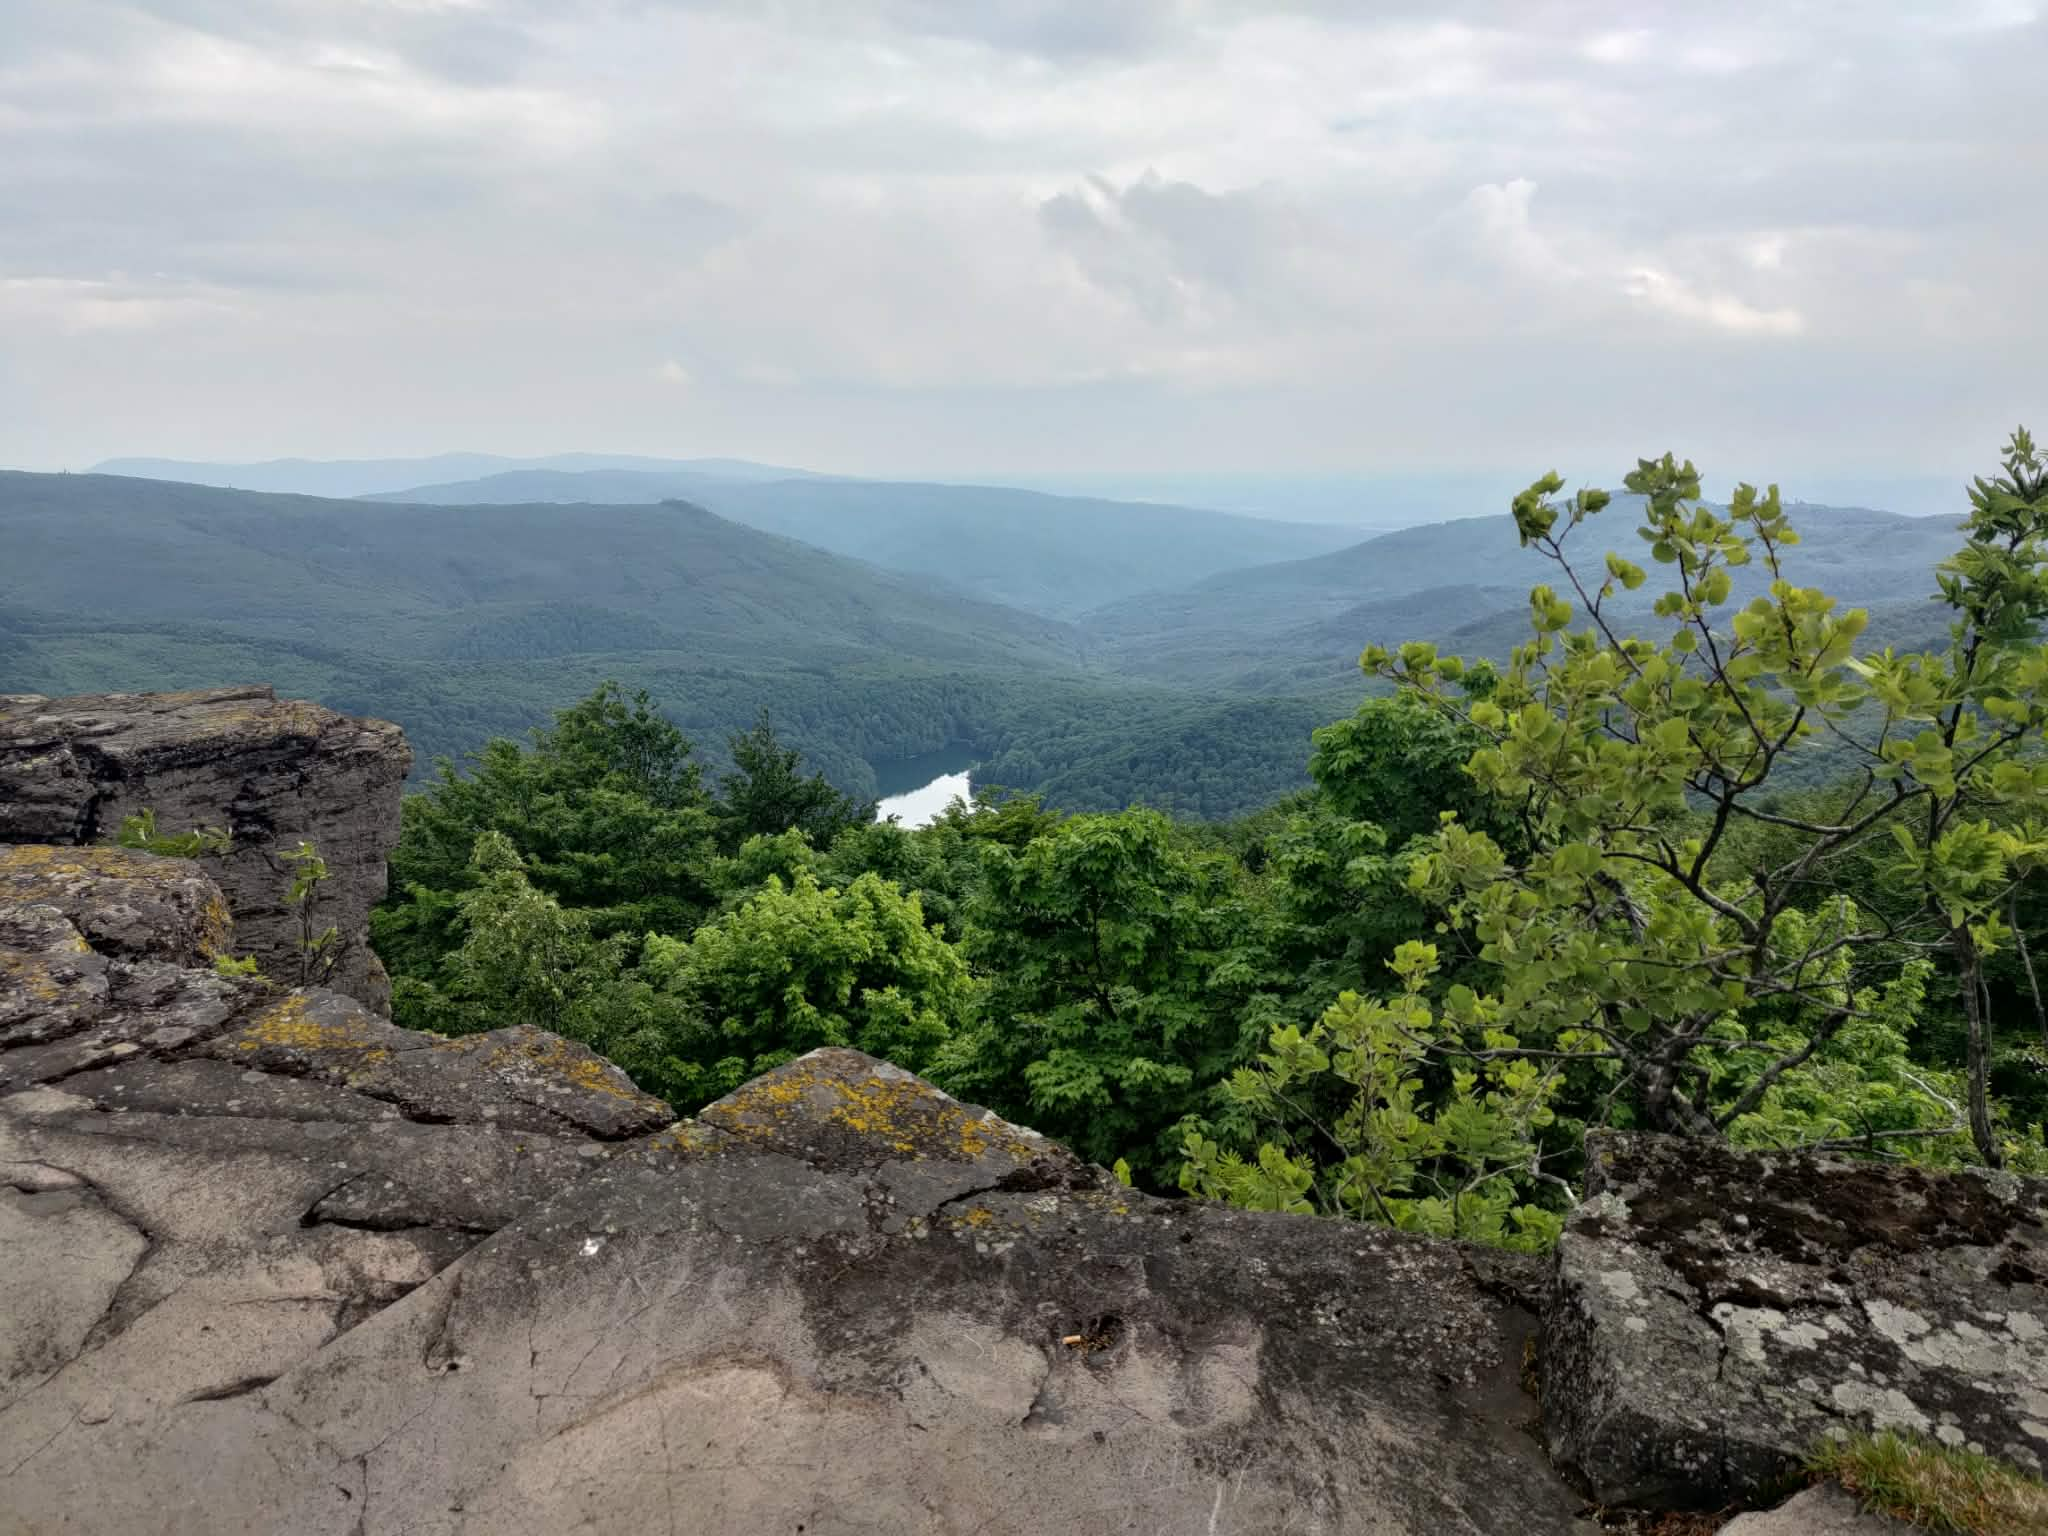
\includegraphics[width=0.50\textwidth]{figures/lake.jpeg}
\end{center}

\vfill

\begin{columns}[c]
    \begin{column}{0.43\textwidth}
        \centering
        
\includegraphics[width=\textwidth]{figures/animal1.jpeg}
    \end{column}
    
    \begin{column}{0.48\textwidth}
        \centering
        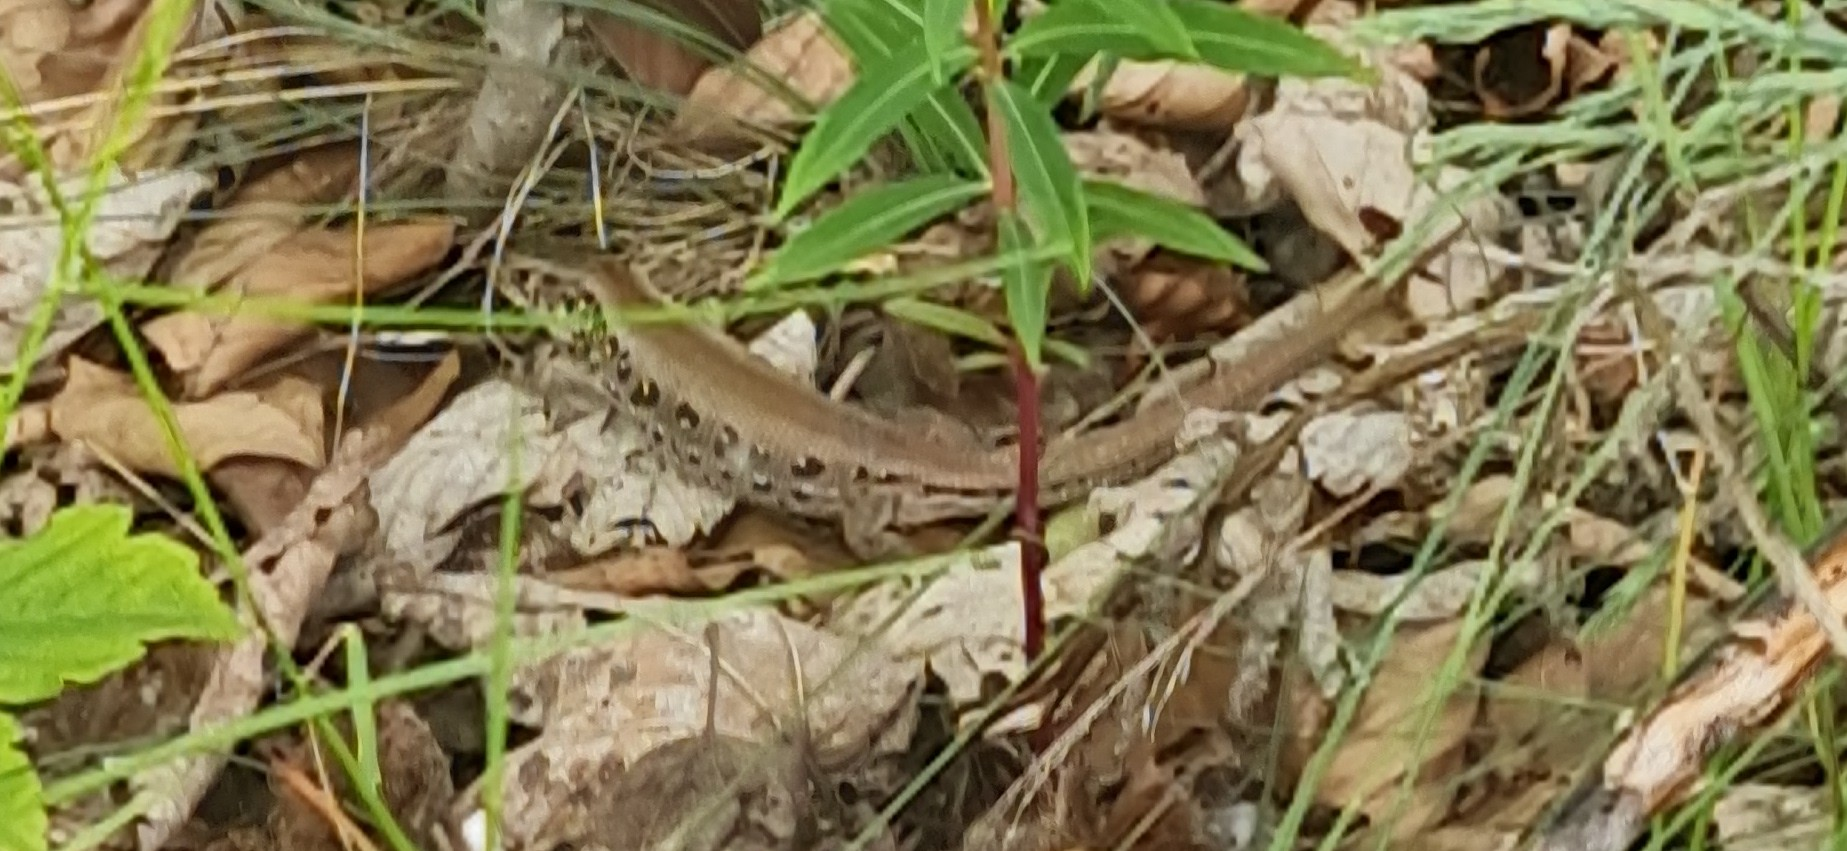
\includegraphics[width=\textwidth]{figures/animal2.jpg}
    \end{column}
\end{columns}
\end{frame}



\begin{frame}{Olympiad in Artificial Intelligence}
\begin{itemize}
    \item \textbf{Date:} April 16 -- April 18, 2026
    \item \textbf{Location:} Pavol Jozef Šafárik University in Košice
    \item \textbf{Event:} The finals of the 1st national Olympiad in Artificial Intelligence
    \item \textbf{Role:} Actively assisted with the organization and smooth running of the competition
\end{itemize}

\vfill

\begin{columns}[c]
    \begin{column}{0.40\textwidth}
        \centering
        
\includegraphics[width=\textwidth]{figures/AI_logo.png}
    \end{column}
    
    \begin{column}{0.58\textwidth}
        \centering
        
\includegraphics[width=\textwidth]{figures/AI_olympiada.png}
    \end{column}
\end{columns}
\end{frame}

\section{Events}

\begin{frame}{Traditional Slovak Cabbage Soup}

\includegraphics[width=1\textwidth]{figures/kapustinca.jpg} 
\end{frame}





\begin{frame}{Collaboration with the Hospital}
\begin{itemize}
    \item \textbf{Partner:} Louis Pasteur University Hospital in Košice (UNLP)
    \item \textbf{Project:} Development of software for automated scheduling and hospital shift optimization
    \item \textbf{Timeline:} Active collaboration established in March 2026
\item \textbf{Current Status:} 
    \begin{itemize}
        \item Initial software design is completed
        \item Consulting with hospital management to validate and approve the proposal
    \end{itemize}
\end{itemize}

\vfill

\begin{center}
    
\includegraphics[width=0.35\textwidth]{figures/logo-unlp.jpg}
\end{center}
\end{frame}






\section{Research}

\begin{frame}{Research -- Current State of Art}

\textbf{1. Automated Hyper-Heuristic (AHD)}
\begin{itemize}
    \item \textbf{FunSearch (DeepMind):} Evolutionary search in functional space generating a single global program \cite{romera2024mathematical}.
    \item \textbf{ReEvo:} Language Hyper-Heuristics (LHH) utilizing "verbal gradients" for code evolution \cite{ye2024reevo}.
\end{itemize}

\vfill

\textbf{2. Post-Optimization via LLMs}
\begin{itemize}
    \item \textbf{DASH:} Co-optimizing search trajectory and runtime schedules \cite{guo2026dynamics}.
    \item \textbf{G-LNS:} Generative Large Neighborhood Search designing static \textit{Destroy} and \textit{Repair} operators \cite{zhao2026g}.
\end{itemize}

\vfill
\begin{block}{\textbf{The Core Shared Limitation}}
All current methods focus on \textbf{global rules} (offline design for the entire problem class), failing to adapt to the features of a \textbf{specific instance}.
\end{block}

\end{frame}

\begin{frame}{Research -- Vision and Objectives}
\textbf{1. Instance-Specific Hyper-Heuristics (HH)}
\begin{itemize}
    \item Shifting from "average-best" global code to context-aware adaptation.
    \item LLM-driven analysis of \textbf{instance attributes} (e.g., edge density, node distribution) in real-time.
    \item Tailoring the algorithmic logic specifically to the graph's structural topology.
    \item Focusing on instance heterogeneity where global methods fail.
\end{itemize}

\vfill
\textbf{2. Hybrid Post-Optimization Pipeline}
\begin{itemize}
    \item Utilizing LLMs to iteratively refine existing sub-optimal solutions.
    \item Improving existing sub-optimal solutions locally instead of generating them from scratch.
\end{itemize}
\end{frame}










\begin{frame}{References}
\scriptsize
\begin{thebibliography}{9}

    \bibitem{romera2024mathematical}
    B. Romera-Paredes et al., "Mathematical discoveries from program search with large language models," \emph{Nature}, vol. 625, no. 7996, pp. 768–775, 2024.

    \bibitem{ye2024reevo}
    H. Ye et al., "ReEvo: Large Language Models as Hyper-Heuristics with Reflective Evolution," \emph{arXiv preprint arXiv:2402.01145}, 2024.

    \bibitem{guo2026dynamics}
    J. Guo et al., "Dynamics-Aware Solver Heuristics (DASH): Co-Optimizing Search and Runtime Schedules," \emph{arXiv preprint arXiv:2601.20868}, 2026.

    \bibitem{zhao2026g}
    B. Zhao et al., "G-LNS: Generative Large Neighborhood Search for LLM-Based Automatic Heuristic Design," \emph{arXiv preprint arXiv:2602.08253}, 2026.

\end{thebibliography}
\end{frame}































\begin{frame}{Thank You}
\vspace{1.5em}
\begin{center}
    \Large Thank you for your attention
\end{center}
\end{frame}










\end{document}
